\section{Diseño}

\subsection{Visión global de la aplicación}

\quad La aplicación consta de tres escenas:\\

\begin{itemize}
	\item Init: donde la aplicación empieza.
	\item EchoChamber: donde se testeó el efecto del eco.
	\item Forest: donde se prueba el efecto del 8D con varios focos de sonido.
\end{itemize}

\quad Antes de empezar a hablar de cada uno de los elementos particulares de cada escena, es imperativo hablar de los elementos que son comunes en todas ellas. De este modo, en toda escena vamos a encontrar una serie de elementos que son imprescindibles: 
\begin{itemize}
	\item Foco de luz: configurado como luz direccional
	\item RealPlayer: contiene la cámara y la retícula y hace la función de representarnos en el mundo virtual
	\item GvrEditorEmulator: encargado de simular con el ratón el movimiento en modo VR
	\item GvrEventSystem: que se encarga de activar el input de colisión entre el rayo de detección que se emite desde la cámara por la retícula y los objetos con los que podemos interaccionar 
	\item SceneManager: se encarga de gestionar los eventos de salir de la aplicación y cambiar de escena
	item GvrControllerMain: se utiliza para determinar controles más allá del giro de cámara y el click, pero al final este elemento no se llegó a utilizar
\end{itemize}

\quad Ahora se pasa a hablar de las particularidades de cada escena.\\

\subsection{Escenas}
	\subsubsection{Init}
\quad Esta escena pretende poner en situación al usuario, indicando con un texto sobre una pared invisible como moverse y que es lo que tiene que hacer en ella.\\

\quad El objetivo será tan simple como encontrar el foco de sonido que lo está llamando. La voz para el foco ha sido aportada por Juan Hernández García, persona que menciono en los agradecimientos.\\

\begin{figure}[htb]
	\centering
	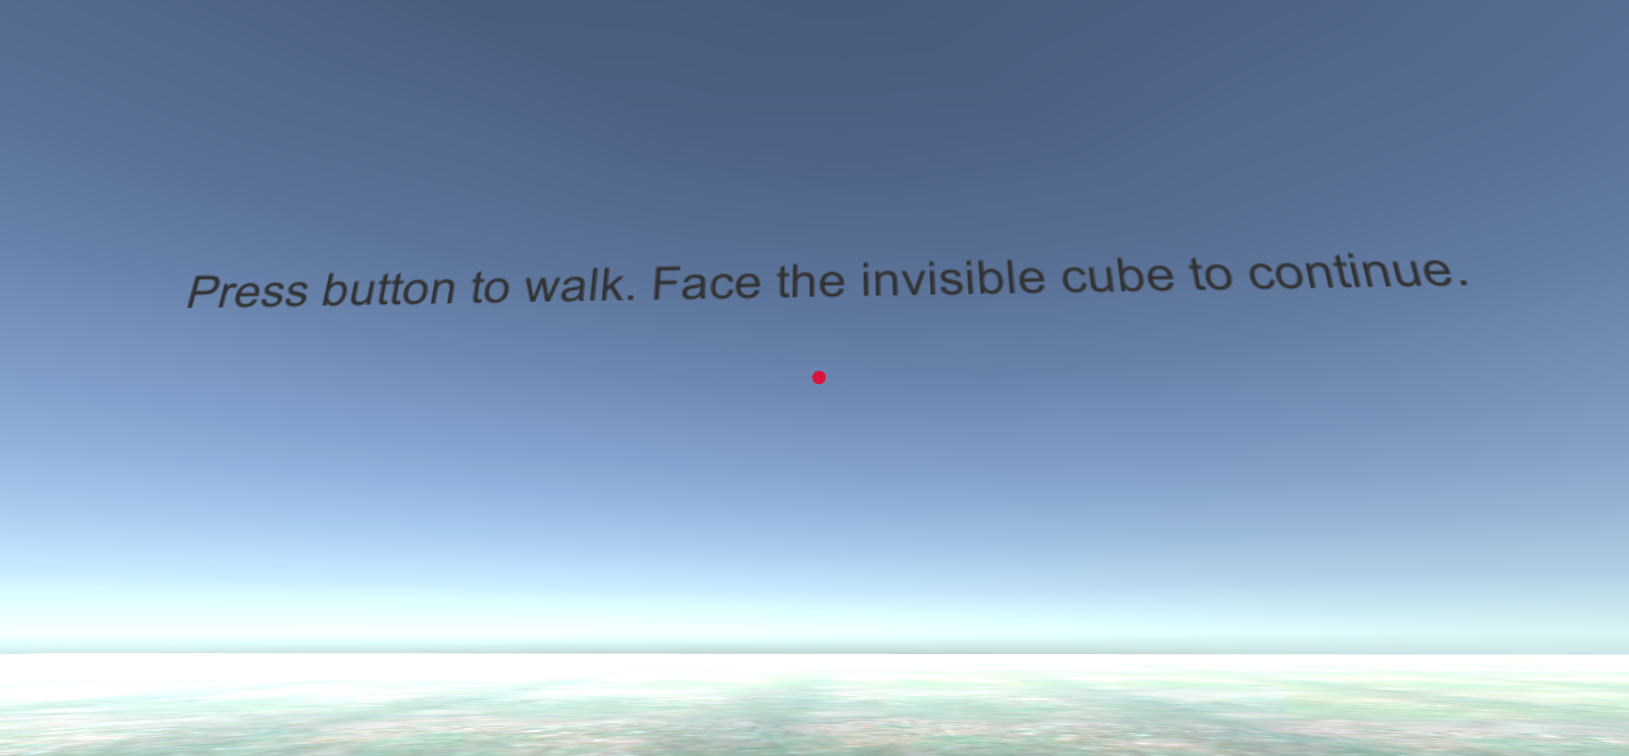
\includegraphics[width=0.6\textwidth]{./imagenes/initInstructions}
	\caption{Instrucciones de uso}
\end{figure}

\begin{figure}[htb]
	\centering
	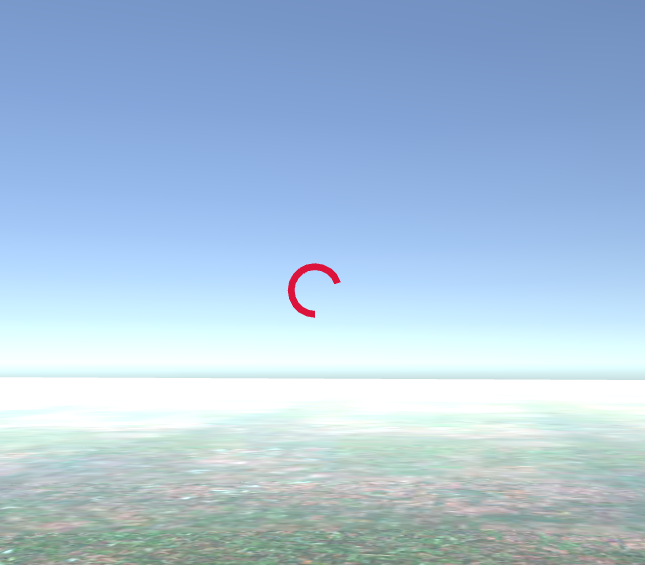
\includegraphics[width=0.248\textwidth]{./imagenes/inactiveCube}
	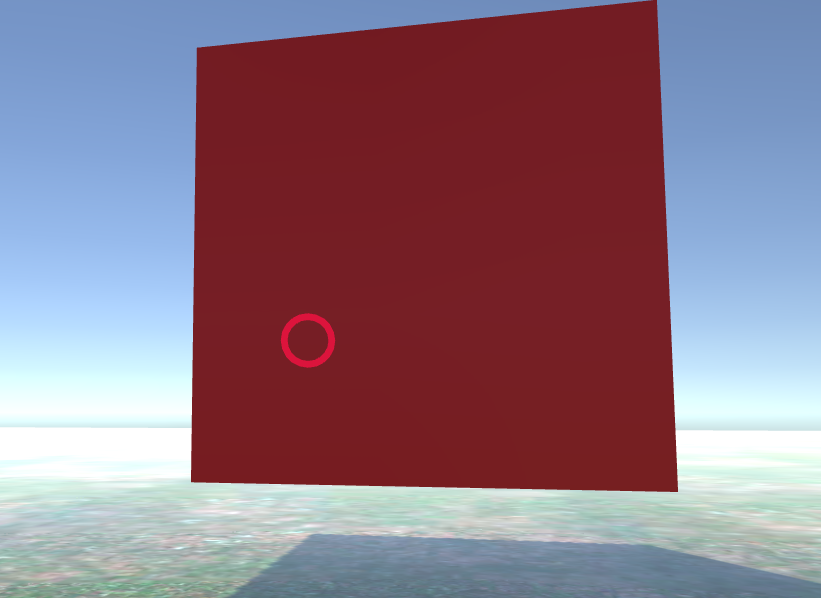
\includegraphics[width=0.3\textwidth]{./imagenes/activeCube}
	\caption{Cubo}
\end{figure}

\subsubsubsection{Componentes de Init}

\quad Dicho todo esto, toca hablar de cada uno de los elementos no comunes de la escena. De este modo, quedan por comentar los siguientes elementos:

\begin{itemize}
	\item Cube: sujeto que que se vuelve visible al encontrar su posición siguiendo el sonido de su llamada
	\item Plane: suelo de la escena
	\item Canvas: contiene un texto en que van unas pequeñas instrucciones
	\item Walls: Se forma con cuatro prismas invisibles que actuarán como muros invisibles para delimitar la zona de movimiento
\end{itemize}

	\subsubsection{EchoChamber}
\quad Esta habitación tiene como objetivo mostrar el efecto del eco ante un foco de sonido, en este caso será un icosaedro que toca la tonadilla libre de derechos \textit{If i had a chicken}, típica canción de taberna del oeste. Este icosaedro se tele transportará a otro lugar de la habitación cuando interactuemos con él.\\

\begin{figure}[htb]
	\centering
	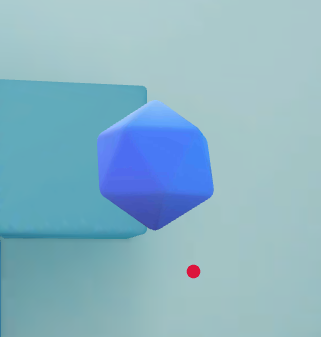
\includegraphics[width=0.4\textwidth]{./imagenes/icosaedroInactivo}
	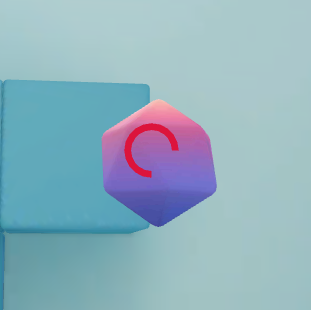
\includegraphics[width=0.4229\textwidth]{./imagenes/icosaedroActivo}
	\caption{Icosaedro sonoro}
\end{figure}

\quad Además, se encontrarán dos menús, unos con dos botones y otro con varios desplegables.\\

\quad Mediante el menú de dos botones se podrá salir de la aplicación o avanzar a la última escena. Además este menú contará con un texto que indique la utilidad de esta escena.\\

\begin{figure}[htb]
	\centering
	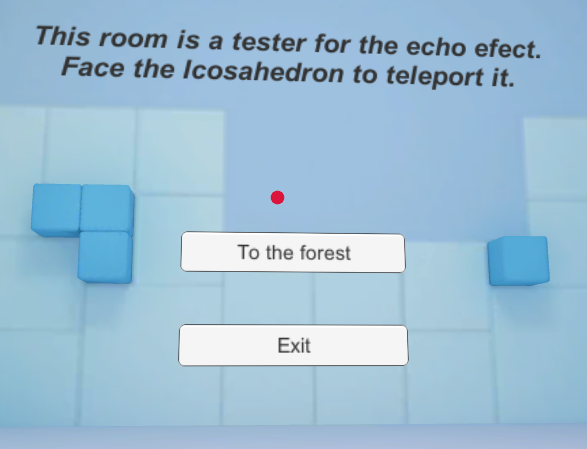
\includegraphics[width=0.5\textwidth]{./imagenes/echoMenu}
	\caption{Menú e instrucciones de la habitación}
\end{figure}

\quad El menú de desplegables se utiliza para para cambiar el tipo de material del que se componen las superficies de la habitación.\\

\begin{figure}[htb]
	\centering
	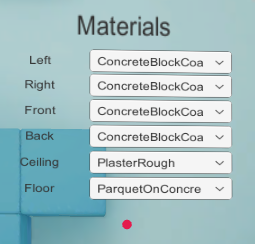
\includegraphics[width=0.3\textwidth]{./imagenes/materialMenu}
	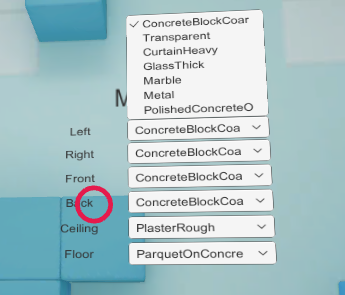
\includegraphics[width=0.3\textwidth]{./imagenes/materialMenuDeploy}
	\caption{Menú para cambio de materiales}
\end{figure}
\FloatBarrier

\subsubsubsection{Componentes de EchoChamber}
	
\quad Los elementos no comunes de la escena EchoChamber determinarán el comportamiento de la misma:
\begin{itemize}
	\item ResonanceAudioRoom: delimita la zona cúbica donde el eco puede trabajar. Si se sale de esta delimitación el eco desaparece
	\item CubeRoom: en esta escena se tiene una escena cúbica que delimita el espacio de interacción
	\item Menu: compuestos por dos botones (uno para avanzar de escena y otro para salir de la aplicación) y un texto que explica cómo funciona la escena.
\item Icosahedron: es el punto de sonido de la escena, y al interaccionar con él se teletransportará a un lugar aleatorio de la escena para poder observar cómo esto afecta al eco de la habitación
\item Canvas: este canvas tiene dentro una serie de dropdown que interaccionan directamente con ResonanceAudioRoom para modificar los diferentes materiales que que componen sus caras.
\end{itemize}

\quad En particular ResonanceAudioRoom, Icosahedron y Canvasson especialmente importantes, pues son los que permiten trabajar con el eco en esta habitación, pero no adelantemos acontecimientos.\\

	\subsubsection{Forest}

\quad Esta escena pretende representar un pequeño bosque lleno de pájaros que van cantando, volando por las cercanías.\\

\quad Dispone de un menú para volver a la escena EchoChamber o salir de la aplicación.\\

\begin{figure}[htb]
	\centering
	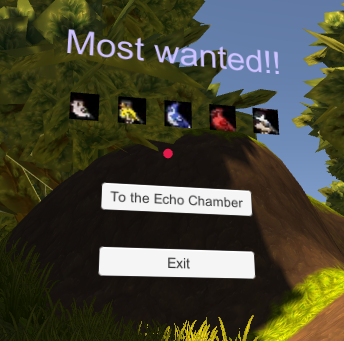
\includegraphics[width=0.36\textwidth]{./imagenes/forestMenu}
	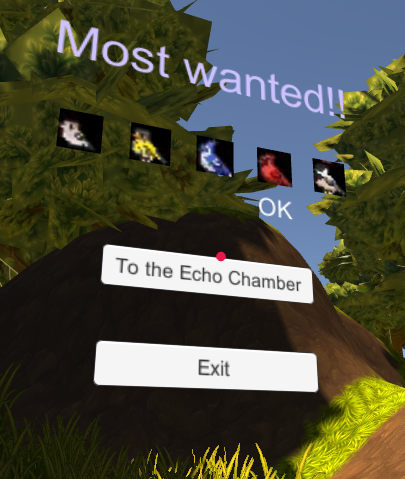
\includegraphics[width=0.38\textwidth]{./imagenes/forestMenuActive}
	\caption{Menú en el bosque}
\end{figure}

\quad En la parte superior del menú se encuentra un banner con los cinco pájaros dentro de la selección que se introduzcan en la aplicación. Cuando se visualice al tipo de pájaro objetivo, se marcará en ese banner.\\

\begin{figure}[htb]
	\centering
	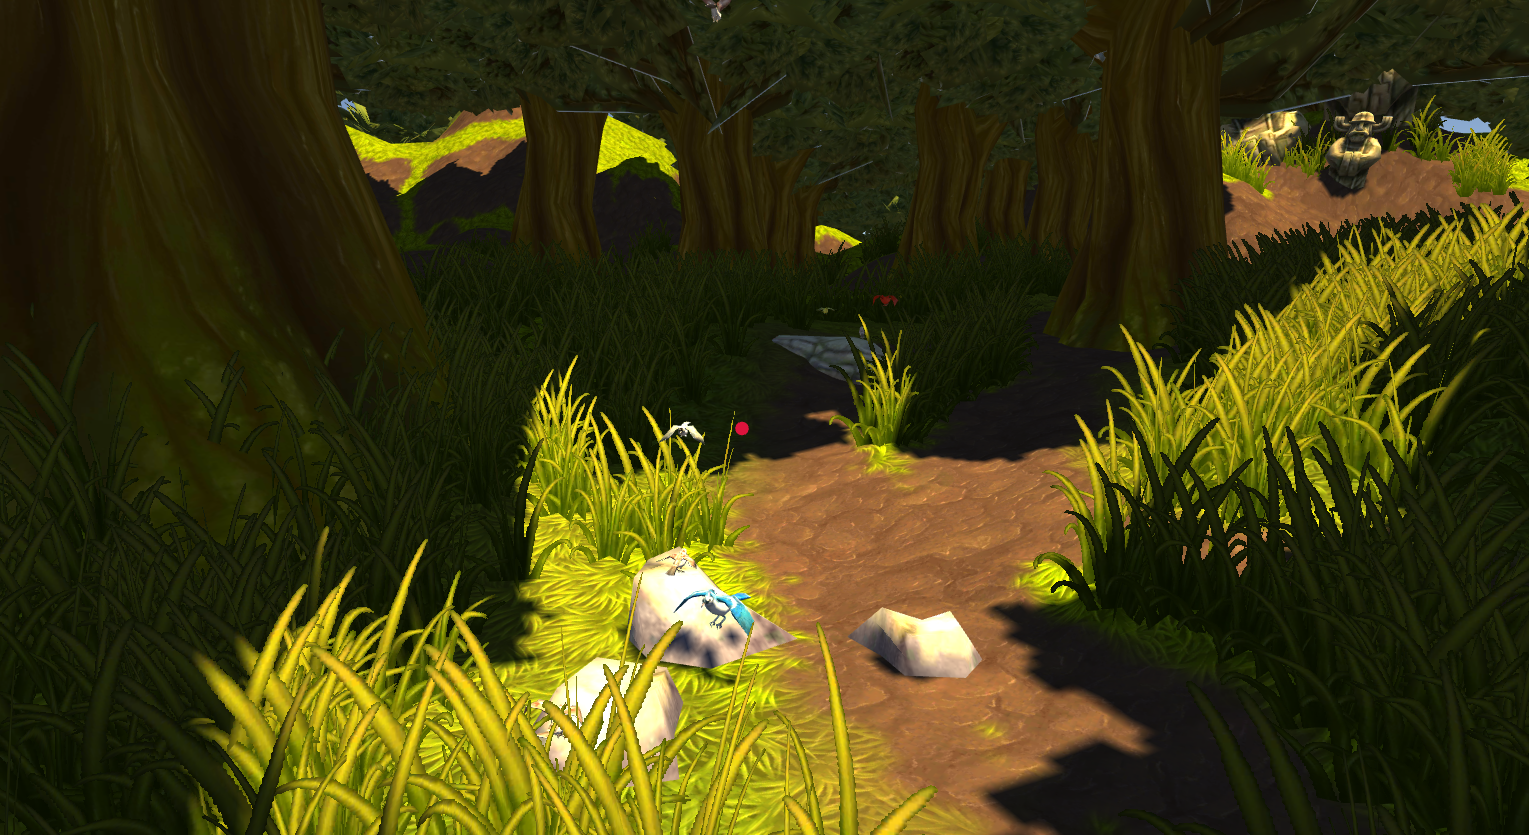
\includegraphics[width=0.7\textwidth]{./imagenes/forestBirds}
	\caption{Pajaros en el bosque}
\end{figure}

\quad Debido a la carga que tendrá esta escena, es importante cambiar shaders y aplicar técnicas de optimización para evitar que la tasa de frames caiga demasiado.

\begin{figure}[htb]
	\centering
	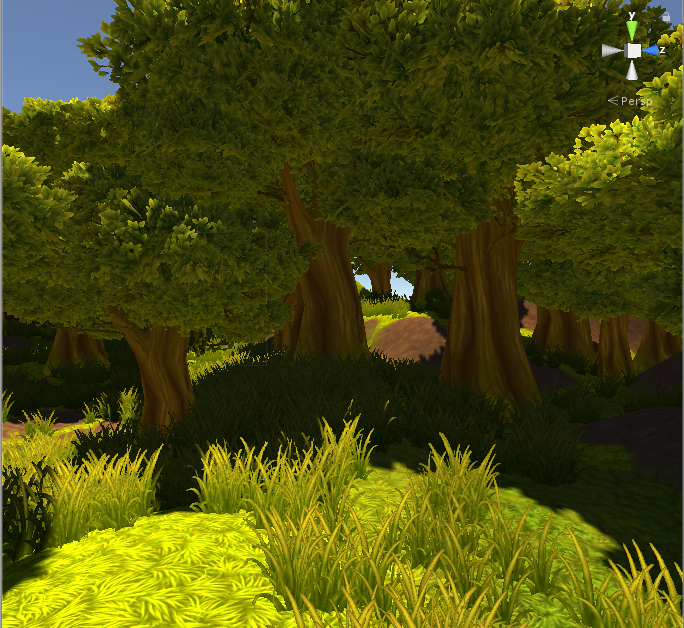
\includegraphics[width=0.45\textwidth]{./imagenes/highShadders}
	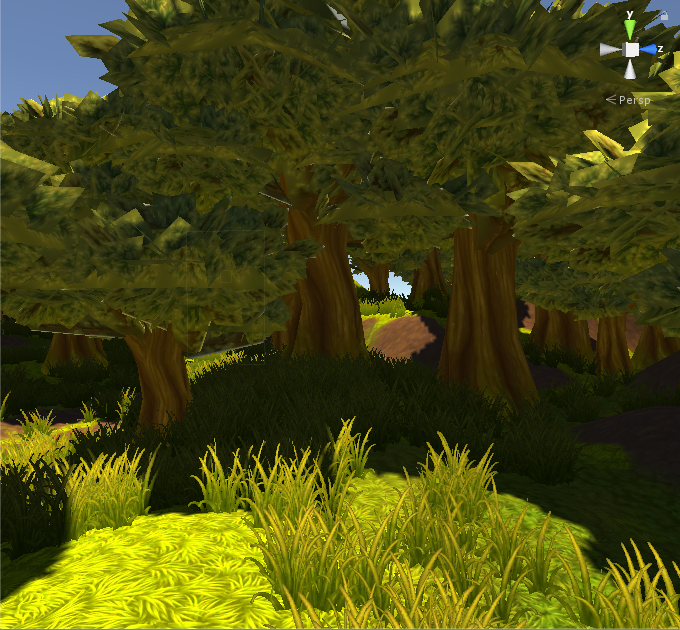
\includegraphics[width=0.45\textwidth]{./imagenes/lowShadders}
	\caption{Comparativa entre shader de alta calidad y baja calidad}
\end{figure}
\FloatBarrier

\subsubsubsection{Componentes de Forest}

\quad Forest es con diferencia la escena con más carga de elementos de todo el proyecto, por lo que voy a diferenciar entre tipos de elementos.\\

\quad Primero debemos se va a hablar de los elementos que tiene que ver con la topografía de las escena:

\begin{itemize}
	\item Terrain: terreno irregular que crearemos utilizando las herramientas de Unity. Aprovechando el asset Fantasy Forest, le agregaremos proceduralmente hierba y árboles
	\item Rock: Utilizaremos los dos tipos de rocas del asset Hand Painted Forest para dar algo de personalidad a nuestro bosque
	\item Statue: utilizaremos los modelados de estatuas del asset anteriormente nombrado para darle más personalidad al bosque
\end{itemize}

\quad Ahora pasamos a ver los elementos asociados al comportamiento de los pájaros:

\begin{itemize}
	\item \_livingBirdsController: se encarga de lanzar los distintos tipos de pájaros para que interaccionen por el bosque
	\item lc\_perchTarget: hace de objetivo donde los pájaros aterrizan, siempre que este no esté en el suelo
	\item lb\_GroundTarget: determina un lugar de aterrizaje para los pájaros en el suelo
\end{itemize}

\quad Una aclaración importante es que lc\_perchTarget y lb\_GroundTarget afectan de manera distinta al árbol de animaciones de los pájaros.\\

\quad Forest posee, al igual que Init, un conjunto de muros invisibles llamado Wall que determina la zona por la que el jugador puede moverse.\\ 

\quad El último tipo de elemento que queda por remarcar es un menú con con las mismas interacciones que tenía el de EchoChamber, pero con una particularidad, posee un banner encima suyo que determina si hemos visto o no los pájaros en el postrado.\\


\newpage





